% =====================================================================
\section{Reproduction of the Paper's Simulations}
\label{sec:repro}
% =====================================================================

The paper validates its controller on a rigid spacecraft in two parts (its Section IV). We repeated both with the
paper's inertia, disturbance, actuator limit, gains, envelopes and initial states (Mathematical Models, Section 2.3).
The paper publishes plots only, so we compare the behaviour of the plots and, in addition, report the metrics of
\cref{sec:metrics}, which make the comparison checkable. All numbers: \code{docs/results/metrics.md}.

% ---------------------------------------------------------------------
\subsection{Part 1: effect of the settling time $T_s$}
\label{sec:part1}
% ---------------------------------------------------------------------

\textbf{Paper's claim.} The quaternion and the angular velocity stay inside $\pm\rho(t)$, the controller does not let the
trajectories touch the boundaries, a smaller $T_s$ gives faster convergence, and the torque stays within the limit.

\begin{figure}[H]
\centering
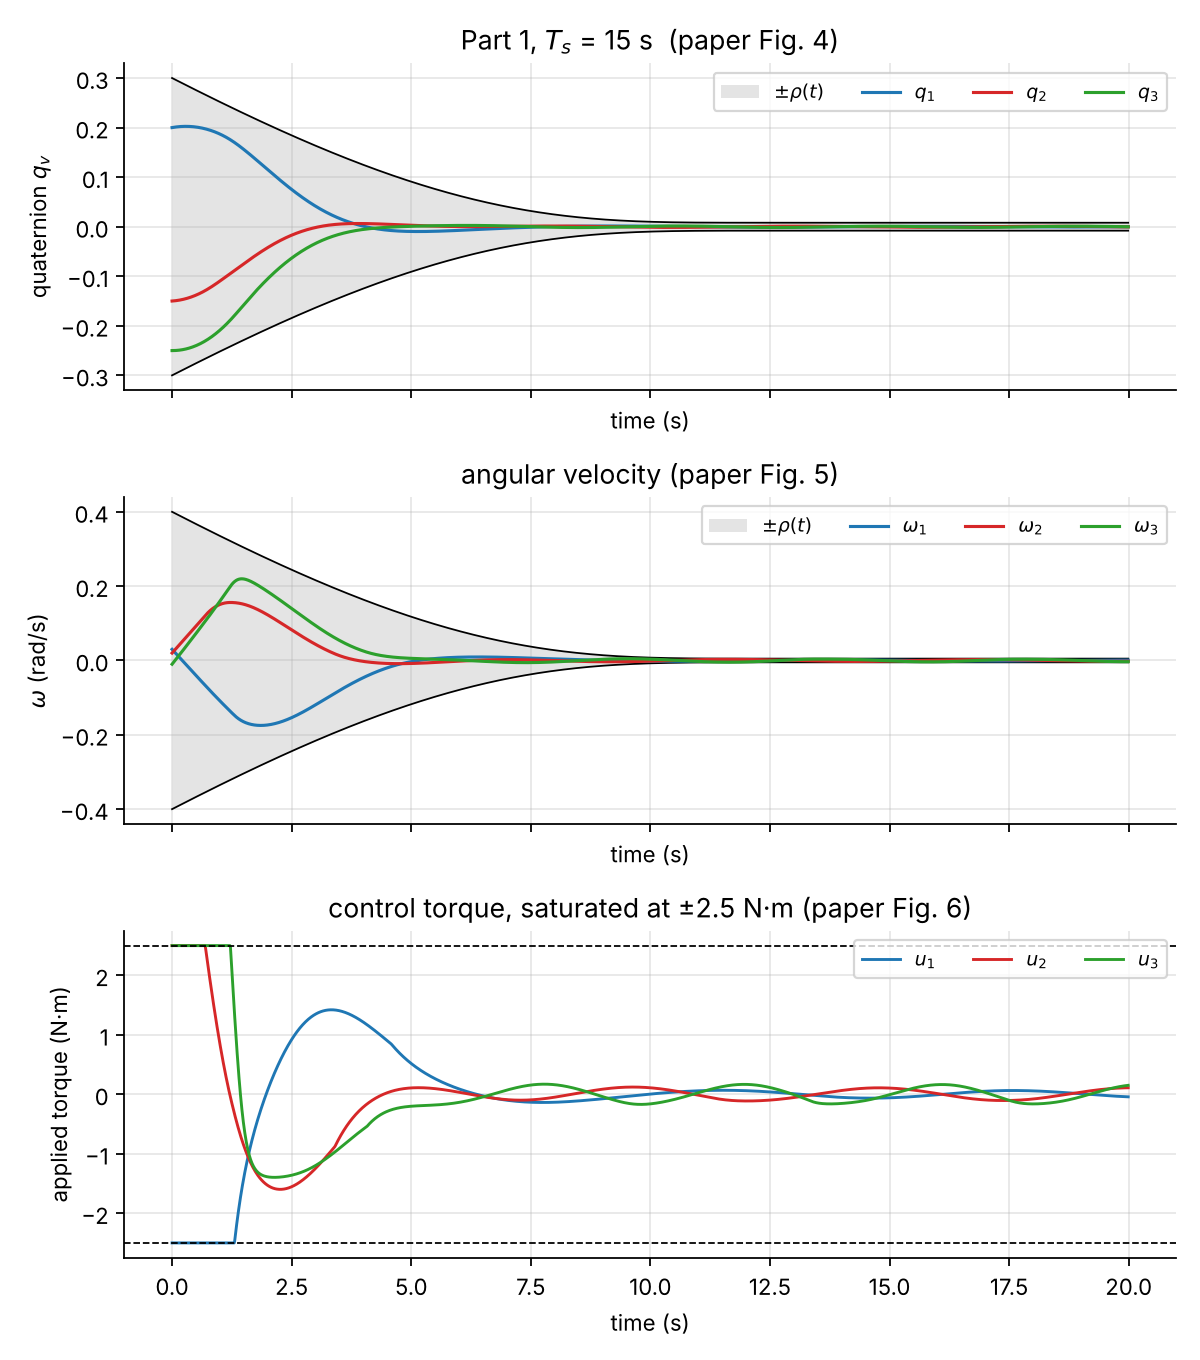
\includegraphics[width=0.49\linewidth]{fig02_part1_Ts15.png}\hfill
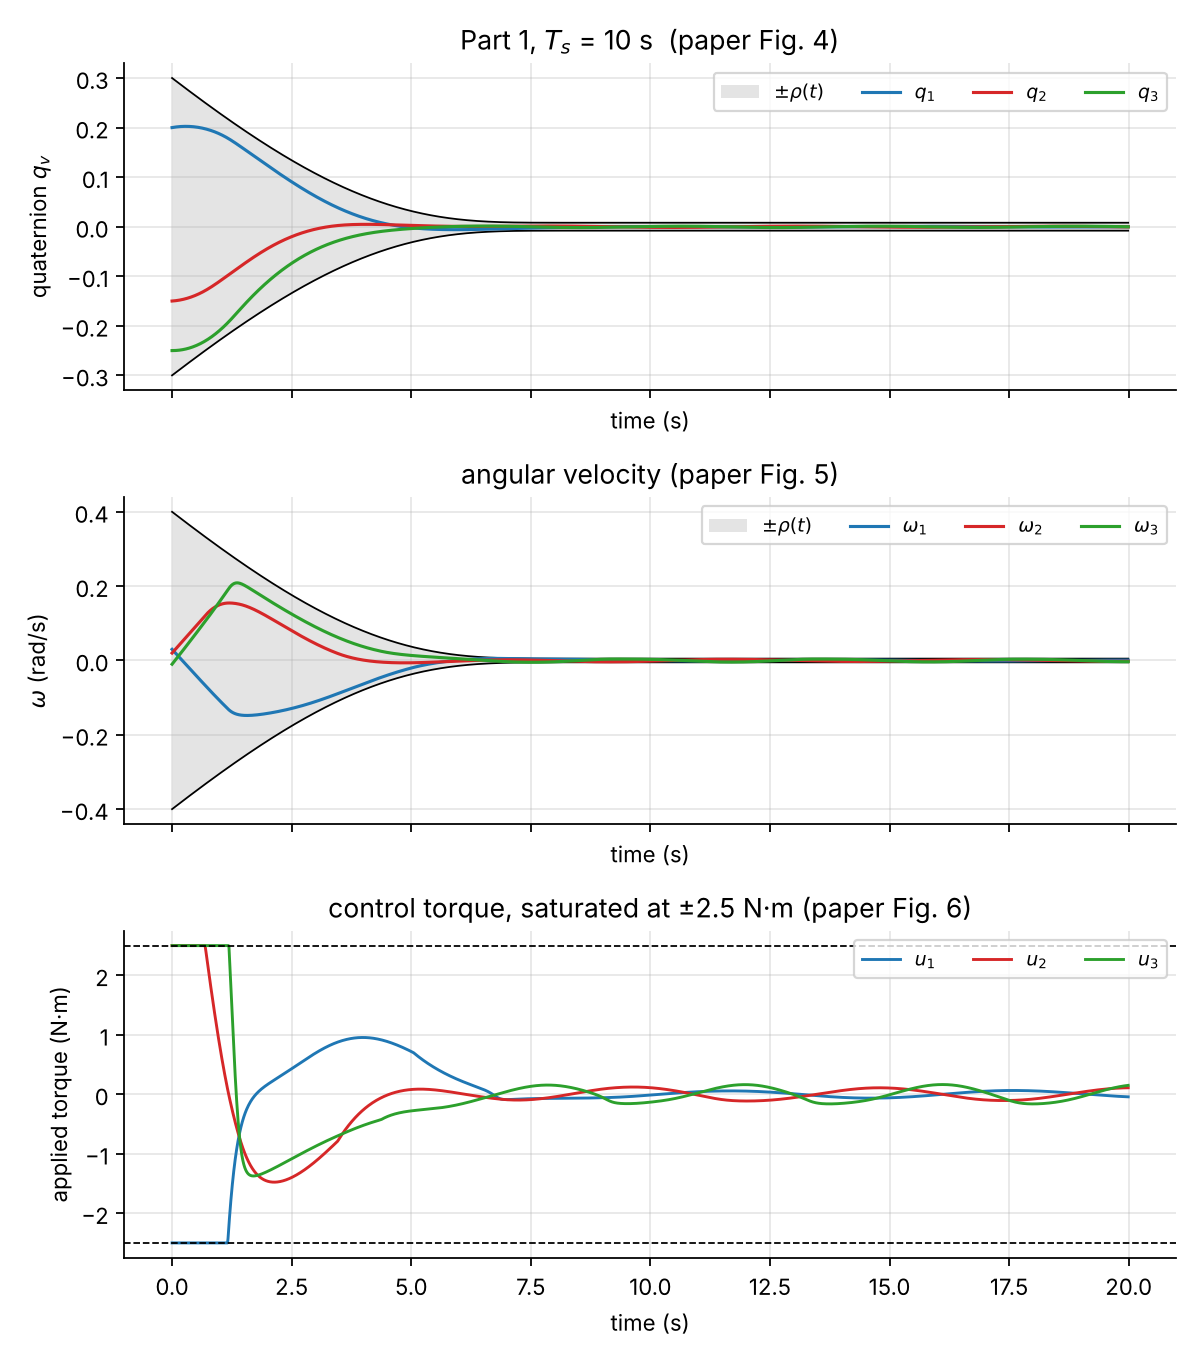
\includegraphics[width=0.49\linewidth]{fig02_part1_Ts10.png}
\caption{Part 1 reproduction, $T_s=15$\,s (left) and $T_s=10$\,s (right). Top: $\qv$ inside $\pm\rho_q$ (paper Fig.~4).
Middle: $\vw$ inside $\pm\rho_\omega$ (paper Fig.~5). Bottom: applied torque, saturated at $\pm2.5$\,N\,m during the first
second (paper Fig.~6).}
\label{fig:part1}
\end{figure}

\begin{table}[H]
\centering\small
\caption{Part 1 metrics (constrained law, paper form).}
\label{tab:part1}
\begin{tabular}{@{}lcc@{}}
\toprule
\textbf{Metric} & $T_s=15$\,s & $T_s=10$\,s\\
\midrule
time outside $\rho_q$ / outside $\rho_\omega$ & 0\,\% / 0\,\% & 0\,\% / 0\,\%\\
$\max|\varepsilon_1|$ / $\max|\varepsilon_2|$ & 0.871 / 0.912 & 0.924 / 0.942\\
settling time ($\|\qv\|<0.01$) & 5.25\,s & 4.53\,s\\
final $\|\qv\|$ / final $\|\vw\|$ (rad/s) & $4.4\times10^{-4}$ / $4.0\times10^{-3}$ & $4.5\times10^{-4}$ / $4.1\times10^{-3}$\\
time with commanded torque at the limit & 6.5\,\% & 5.9\,\%\\
peak commanded torque (before saturation) & 10.54\,N\,m & 10.54\,N\,m\\
$\that$ at 20\,s & 0.433 & 0.416\\
\bottomrule
\end{tabular}
\end{table}

\resfig{fig03_part1_convergence.png}{0.95\linewidth}{Convergence on a log scale: with $T_s=10$\,s both $\|\qv\|$ and $\|\vw\|$
fall faster during the transient. After the envelope has closed, both runs settle on the same small residual set by the
disturbance and the boundary layer.}{fig:part1conv}

\begin{projbox}[result]
Every statement of Part~1 is reproduced: 0\,\% of the time outside either envelope for both settling times, the largest
normalised error is 0.942 (6\,\% margin to the wall), the shorter $T_s$ settles 0.72\,s earlier, and the applied torque
never exceeds 2.5\,N\,m (it saturates only in the first $\approx1.2$\,s, when the initial error is largest). The peak of the
\emph{commanded} torque (10.54\,N\,m, at $t=0$) is the value computed by hand in the Mathematical Models (block 5).
\end{projbox}

% ---------------------------------------------------------------------
\subsection{Part 2: constrained PD-type versus conventional PD}
\label{sec:part2}
% ---------------------------------------------------------------------

\textbf{Paper's claim.} With the same maximum control torque, the constrained law keeps both states inside their
envelopes, whereas conventional PD is ``not capable of providing as fast and accurate convergence''.

\textbf{Set-up.} Both controllers have the same $k_p=40$, $k_d=20$, the same 2.5\,N\,m limit, the same disturbance and
the same initial state $\vq(0)=[0.3,-0.2,-0.3,0.8832]$, $\vw(0)=[-0.02,-0.02,0.025]$\,rad/s; conventional PD is the law
with $\vu_{cons}=0$. $T_s=15$\,s and $\rho_{q0}=0.36$ (the paper's 0.3 would put the initial state on the boundary).

\resfig{fig04_part2_quaternion.png}{0.92\linewidth}{Part 2, quaternion (paper Fig.~7). Both controllers keep $\qv$ inside
$\pm\rho_q$ in this run.}{fig:part2q}

\resfig{fig05_part2_angular_velocity.png}{0.92\linewidth}{Part 2, angular velocity (paper Fig.~8). Black dots: conventional
PD outside $\pm\rho_\omega$, both during the transient ($t\approx2$\,s, axes 1 and 3) and in steady state, where the
disturbance keeps $|\omega_3|$ above $\rho_{\omega T}=0.005$\,rad/s. The constrained law stays inside throughout.}{fig:part2w}

\resfig{fig06_part2_torque.png}{0.95\linewidth}{Part 2, applied torque (paper Fig.~9). Both controllers use the same maximum
torque, 2.5\,N\,m, as in the paper.}{fig:part2u}

\resfig{fig07_part2_normalised_error.png}{0.95\linewidth}{The clearest view of the constraint: $\max_i|\varepsilon_{1i}|$ and
$\max_i|\varepsilon_{2i}|$. Below the red line means inside. Conventional PD crosses it for the angular velocity.}{fig:part2eps}

\begin{table}[H]
\centering\small
\setlength{\tabcolsep}{3.5pt}
\caption{Part 2 metrics ($T_s=15$\,s, $\rho_{q0}=0.36$; same gains, limit, disturbance and initial state).}
\label{tab:part2}
\footnotesize
\begin{tabular}{@{}lccc@{}}
\toprule
\textbf{Metric} & \textbf{constrained (paper)} & \textbf{constrained (symm.)} & \textbf{conventional PD}\\
\midrule
time outside $\rho_q$ & 0\,\% & 0\,\% & 0\,\%\\
time outside $\rho_\omega$ & \textbf{0\,\%} & \textbf{0\,\%} & \textbf{27.5\,\%}\\
$\max|\varepsilon_1|$ / $\max|\varepsilon_2|$ & 0.868 / 0.904 & 0.868 / 0.837 & 0.868 / 1.496\\
time with commanded torque at the limit & 6.3\,\% & 7.2\,\% & 14.0\,\%\\
peak commanded torque & 18.8\,N\,m & 13.8\,N\,m & 11.6\,N\,m\\
settling time ($\|\qv\|<0.01$) & 5.79\,s & 4.19\,s & 6.31\,s\\
final $\|\vw\|$ (rad/s) & 0.0040 & 0.0040 & 0.0083\\
final $\|\qv\|$ & $4.4\times10^{-4}$ & $3.9\times10^{-4}$ & $9.0\times10^{-4}$\\
torque energy $\int\|\sat(\vu)\|^2dt$ & 38.9 & 41.5 & 60.5\\
final $\that$ & 0.439 & 0.435 & --\\
\bottomrule
\end{tabular}
\end{table}

\begin{projbox}[result]
The central claim of the paper is reproduced. At the same 2.5\,N\,m limit the constrained law keeps the angular velocity
inside its envelope all the time, conventional PD is outside 27.5\,\% of the time (peak $|\varepsilon_2|=1.50$). The
constrained law also settles earlier (5.79 vs.\ 6.31\,s), ends with half the rate error (0.0040 vs.\ 0.0083\,rad/s) and less
than half the attitude error, spends less than half as much time at the torque limit (6.3 vs.\ 14.0\,\%) and uses 36\,\%
less torque energy.
\end{projbox}

\begin{warn}[Reading Part 2 fairly]
In this run the conventional PD also keeps the \emph{quaternion} inside its envelope; the advantage of the constrained
law is in the angular velocity, the residual error and the control effort. The constrained law commands a higher
\emph{peak} torque (18.8\,N\,m) for an instant, but the actuator delivers at most 2.5\,N\,m to both, which is exactly the
paper's ``same maximum control effort''.
\end{warn}

\subsection{Adaptive estimate and Lyapunov function}

\resfig{fig08_theta_hat_and_lyapunov.png}{0.95\linewidth}{Left: $\that(t)$, Eq.~(14). It rises while $\|\vs\|$ is large, drops
when the leakage $\eta_2$ is still strong, and then creeps upwards because $\eta_2=2e^{-0.5t}$ has almost vanished while a
small residual $\|\vs\|$ remains (Mathematical Models, block 6). Right: the state part $V_x$ of the Lyapunov function (15) along the
Part~2 trajectory. It falls by five orders of magnitude within 9\,s and then stays near $10^{-4}$, a floor set by the
persistent disturbance and the boundary layer (ultimate boundedness rather than exact convergence; Mathematical
Models, Theorem~1). The $\ttil$ part of (15) cannot be plotted because the true bound $\theta$ is unknown.}{fig:theta}

% ---------------------------------------------------------------------
\subsection{Independent cross-check in MATLAB}
\label{sec:crosscheck}
% ---------------------------------------------------------------------

\code{toy\_model/step6\_spacecraft\_closed\_loop.m} is a second implementation of the same experiments in a different language, with its own RK4
integrator and its own control law (\code{lib/control\_law.m}); only the equations and parameters are shared.
% generated by docs/make_crosscheck.py - do not edit by hand
\cref{tab:crosscheck} compares the two implementations metric by metric.
\begin{table}[H]
\centering\small
\caption{Cross-check: Python (\code{paper\_reproduction.py}) vs.\ MATLAB (\code{toy\_model/step6}).}
\label{tab:crosscheck}
\begin{tabular}{@{}llcc@{}}
\toprule
\textbf{Case} & \textbf{Metric} & \textbf{Python} & \textbf{MATLAB}\\
\midrule
Part 1, $T_s=15$\,s & $\max|\varepsilon_1|$ & 0.871 & 0.871\\
 & $\max|\varepsilon_2|$ & 0.912 & 0.912\\
 & time outside $\rho_q$ (\%) & 0.0 & 0.0\\
 & time outside $\rho_\omega$ (\%) & 0.0 & 0.0\\
 & settling time (s) & 5.25 & 5.25\\
Part 1, $T_s=10$\,s & $\max|\varepsilon_1|$ & 0.924 & 0.924\\
 & $\max|\varepsilon_2|$ & 0.941 & 0.942\\
 & time outside $\rho_q$ (\%) & 0.0 & 0.0\\
 & time outside $\rho_\omega$ (\%) & 0.0 & 0.0\\
 & settling time (s) & 4.53 & 4.53\\
Part 2, paper form & $\max|\varepsilon_2|$ & 0.904 & 0.904\\
 & time outside $\rho_\omega$ (\%) & 0.0 & 0.0\\
 & time at torque limit (\%) & 6.3 & 6.3\\
 & settling time (s) & 5.79 & 5.79\\
 & torque energy & 38.9 & 38.9\\
Part 2, symmetric & $\max|\varepsilon_2|$ & 0.837 & 0.837\\
 & time outside $\rho_\omega$ (\%) & 0.0 & 0.0\\
 & time at torque limit (\%) & 7.2 & 7.2\\
 & settling time (s) & 4.19 & 4.19\\
 & torque energy & 41.5 & 41.5\\
Part 2, conv.\ PD & $\max|\varepsilon_2|$ & 1.496 & 1.496\\
 & time outside $\rho_\omega$ (\%) & 27.5 & 27.5\\
 & time at torque limit (\%) & 14.0 & 14.0\\
 & settling time (s) & 6.31 & 6.31\\
 & torque energy & 60.5 & 60.5\\
\bottomrule
\end{tabular}
\end{table}
The largest difference over all 25 entries is 0.001 (in the units of the metric).

